% Options for packages loaded elsewhere
\PassOptionsToPackage{unicode}{hyperref}
\PassOptionsToPackage{hyphens}{url}
%
\documentclass[
]{article}
\usepackage{amsmath,amssymb}
\usepackage{lmodern}
\usepackage{iftex}
\ifPDFTeX
  \usepackage[T1]{fontenc}
  \usepackage[utf8]{inputenc}
  \usepackage{textcomp} % provide euro and other symbols
\else % if luatex or xetex
  \usepackage{unicode-math}
  \defaultfontfeatures{Scale=MatchLowercase}
  \defaultfontfeatures[\rmfamily]{Ligatures=TeX,Scale=1}
\fi
% Use upquote if available, for straight quotes in verbatim environments
\IfFileExists{upquote.sty}{\usepackage{upquote}}{}
\IfFileExists{microtype.sty}{% use microtype if available
  \usepackage[]{microtype}
  \UseMicrotypeSet[protrusion]{basicmath} % disable protrusion for tt fonts
}{}
\makeatletter
\@ifundefined{KOMAClassName}{% if non-KOMA class
  \IfFileExists{parskip.sty}{%
    \usepackage{parskip}
  }{% else
    \setlength{\parindent}{0pt}
    \setlength{\parskip}{6pt plus 2pt minus 1pt}}
}{% if KOMA class
  \KOMAoptions{parskip=half}}
\makeatother
\usepackage{xcolor}
\IfFileExists{xurl.sty}{\usepackage{xurl}}{} % add URL line breaks if available
\IfFileExists{bookmark.sty}{\usepackage{bookmark}}{\usepackage{hyperref}}
\hypersetup{
  pdftitle={HW1\_zs2539},
  hidelinks,
  pdfcreator={LaTeX via pandoc}}
\urlstyle{same} % disable monospaced font for URLs
\usepackage[margin=1in]{geometry}
\usepackage{color}
\usepackage{fancyvrb}
\newcommand{\VerbBar}{|}
\newcommand{\VERB}{\Verb[commandchars=\\\{\}]}
\DefineVerbatimEnvironment{Highlighting}{Verbatim}{commandchars=\\\{\}}
% Add ',fontsize=\small' for more characters per line
\usepackage{framed}
\definecolor{shadecolor}{RGB}{248,248,248}
\newenvironment{Shaded}{\begin{snugshade}}{\end{snugshade}}
\newcommand{\AlertTok}[1]{\textcolor[rgb]{0.94,0.16,0.16}{#1}}
\newcommand{\AnnotationTok}[1]{\textcolor[rgb]{0.56,0.35,0.01}{\textbf{\textit{#1}}}}
\newcommand{\AttributeTok}[1]{\textcolor[rgb]{0.77,0.63,0.00}{#1}}
\newcommand{\BaseNTok}[1]{\textcolor[rgb]{0.00,0.00,0.81}{#1}}
\newcommand{\BuiltInTok}[1]{#1}
\newcommand{\CharTok}[1]{\textcolor[rgb]{0.31,0.60,0.02}{#1}}
\newcommand{\CommentTok}[1]{\textcolor[rgb]{0.56,0.35,0.01}{\textit{#1}}}
\newcommand{\CommentVarTok}[1]{\textcolor[rgb]{0.56,0.35,0.01}{\textbf{\textit{#1}}}}
\newcommand{\ConstantTok}[1]{\textcolor[rgb]{0.00,0.00,0.00}{#1}}
\newcommand{\ControlFlowTok}[1]{\textcolor[rgb]{0.13,0.29,0.53}{\textbf{#1}}}
\newcommand{\DataTypeTok}[1]{\textcolor[rgb]{0.13,0.29,0.53}{#1}}
\newcommand{\DecValTok}[1]{\textcolor[rgb]{0.00,0.00,0.81}{#1}}
\newcommand{\DocumentationTok}[1]{\textcolor[rgb]{0.56,0.35,0.01}{\textbf{\textit{#1}}}}
\newcommand{\ErrorTok}[1]{\textcolor[rgb]{0.64,0.00,0.00}{\textbf{#1}}}
\newcommand{\ExtensionTok}[1]{#1}
\newcommand{\FloatTok}[1]{\textcolor[rgb]{0.00,0.00,0.81}{#1}}
\newcommand{\FunctionTok}[1]{\textcolor[rgb]{0.00,0.00,0.00}{#1}}
\newcommand{\ImportTok}[1]{#1}
\newcommand{\InformationTok}[1]{\textcolor[rgb]{0.56,0.35,0.01}{\textbf{\textit{#1}}}}
\newcommand{\KeywordTok}[1]{\textcolor[rgb]{0.13,0.29,0.53}{\textbf{#1}}}
\newcommand{\NormalTok}[1]{#1}
\newcommand{\OperatorTok}[1]{\textcolor[rgb]{0.81,0.36,0.00}{\textbf{#1}}}
\newcommand{\OtherTok}[1]{\textcolor[rgb]{0.56,0.35,0.01}{#1}}
\newcommand{\PreprocessorTok}[1]{\textcolor[rgb]{0.56,0.35,0.01}{\textit{#1}}}
\newcommand{\RegionMarkerTok}[1]{#1}
\newcommand{\SpecialCharTok}[1]{\textcolor[rgb]{0.00,0.00,0.00}{#1}}
\newcommand{\SpecialStringTok}[1]{\textcolor[rgb]{0.31,0.60,0.02}{#1}}
\newcommand{\StringTok}[1]{\textcolor[rgb]{0.31,0.60,0.02}{#1}}
\newcommand{\VariableTok}[1]{\textcolor[rgb]{0.00,0.00,0.00}{#1}}
\newcommand{\VerbatimStringTok}[1]{\textcolor[rgb]{0.31,0.60,0.02}{#1}}
\newcommand{\WarningTok}[1]{\textcolor[rgb]{0.56,0.35,0.01}{\textbf{\textit{#1}}}}
\usepackage{graphicx}
\makeatletter
\def\maxwidth{\ifdim\Gin@nat@width>\linewidth\linewidth\else\Gin@nat@width\fi}
\def\maxheight{\ifdim\Gin@nat@height>\textheight\textheight\else\Gin@nat@height\fi}
\makeatother
% Scale images if necessary, so that they will not overflow the page
% margins by default, and it is still possible to overwrite the defaults
% using explicit options in \includegraphics[width, height, ...]{}
\setkeys{Gin}{width=\maxwidth,height=\maxheight,keepaspectratio}
% Set default figure placement to htbp
\makeatletter
\def\fps@figure{htbp}
\makeatother
\setlength{\emergencystretch}{3em} % prevent overfull lines
\providecommand{\tightlist}{%
  \setlength{\itemsep}{0pt}\setlength{\parskip}{0pt}}
\setcounter{secnumdepth}{-\maxdimen} % remove section numbering
\ifLuaTeX
  \usepackage{selnolig}  % disable illegal ligatures
\fi

\title{HW1\_zs2539}
\author{}
\date{\vspace{-2.5em}2022-09-23}

\begin{document}
\maketitle

\hypertarget{problem-1-solution}{%
\section{Problem 1 Solution}\label{problem-1-solution}}

The dataset penguins includes three specices located in three islands
during 2007-2009, 344 samples in total, describing their bill depth and
length, flipper length, body mass and sex.

\hypertarget{the-size-of-the-dataset-is-as-follows}{%
\subsection{The size of the dataset is as
follows}\label{the-size-of-the-dataset-is-as-follows}}

\begin{itemize}
\tightlist
\item
  Number of Rows
\end{itemize}

\begin{Shaded}
\begin{Highlighting}[]
\FunctionTok{nrow}\NormalTok{(penguins)}
\end{Highlighting}
\end{Shaded}

\begin{verbatim}
## [1] 344
\end{verbatim}

\begin{itemize}
\tightlist
\item
  Number of Columns
\end{itemize}

\begin{Shaded}
\begin{Highlighting}[]
\FunctionTok{ncol}\NormalTok{(penguins)}
\end{Highlighting}
\end{Shaded}

\begin{verbatim}
## [1] 8
\end{verbatim}

\hypertarget{mean-of-flipper-length-in-mm}{%
\subsection{Mean of flipper length in
mm}\label{mean-of-flipper-length-in-mm}}

\begin{Shaded}
\begin{Highlighting}[]
\FunctionTok{mean}\NormalTok{(penguins}\SpecialCharTok{$}\NormalTok{flipper\_length\_mm,}\AttributeTok{na.rm =}\NormalTok{ T)}
\end{Highlighting}
\end{Shaded}

\begin{verbatim}
## [1] 200.9152
\end{verbatim}

\hypertarget{scatterplot-of-flipper-length-bill-length-by-species}{%
\subsection{Scatterplot of Flipper length-Bill Length by
Species}\label{scatterplot-of-flipper-length-bill-length-by-species}}

\begin{Shaded}
\begin{Highlighting}[]
\NormalTok{FBplot1 }\OtherTok{=} \FunctionTok{ggplot}\NormalTok{(}\AttributeTok{data =}\NormalTok{ penguins, }\AttributeTok{mapping =} \FunctionTok{aes}\NormalTok{(}\AttributeTok{x =}\NormalTok{ bill\_length\_mm, }\AttributeTok{y =}\NormalTok{ flipper\_length\_mm, }\AttributeTok{colour =}\NormalTok{ species)) }\SpecialCharTok{+} \FunctionTok{geom\_point}\NormalTok{()}
\NormalTok{FBplot1}
\end{Highlighting}
\end{Shaded}

\begin{verbatim}
## Warning: Removed 2 rows containing missing values (geom_point).
\end{verbatim}

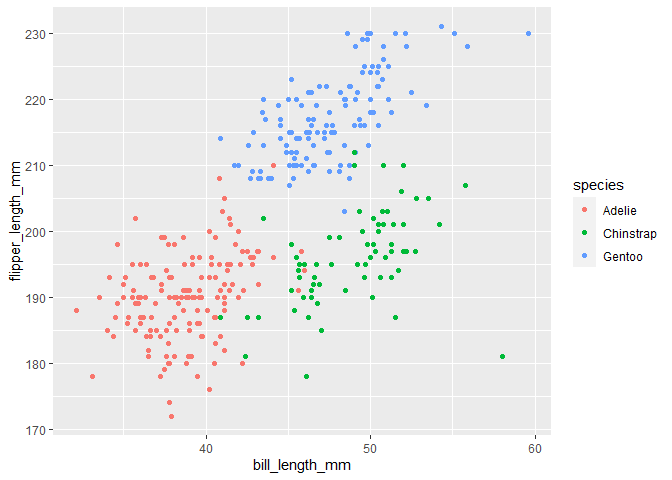
\includegraphics{p8105_hw1_zs2539_files/figure-latex/unnamed-chunk-4-1.pdf}

\hypertarget{export-the-scatterplot-to-the-project-directory}{%
\subsection{Export the scatterplot to the project
directory}\label{export-the-scatterplot-to-the-project-directory}}

\begin{Shaded}
\begin{Highlighting}[]
\FunctionTok{ggsave}\NormalTok{(}\StringTok{"p8105\_hw1\_zs2539.pdf"}\NormalTok{,FBplot1)}
\end{Highlighting}
\end{Shaded}

\begin{verbatim}
## Saving 6.5 x 4.5 in image
\end{verbatim}

\begin{verbatim}
## Warning: Removed 2 rows containing missing values (geom_point).
\end{verbatim}

\hypertarget{problem-2-solution}{%
\section{Problem 2 Solution}\label{problem-2-solution}}

\hypertarget{create-the-data-frame-comprised-of-a-required-random-sample-with-vectors-including-logical-character-and-factor.}{%
\subsection{Create the data frame comprised of a required random sample,
with vectors including logical, character and
factor.}\label{create-the-data-frame-comprised-of-a-required-random-sample-with-vectors-including-logical-character-and-factor.}}

\begin{Shaded}
\begin{Highlighting}[]
\FunctionTok{set.seed}\NormalTok{(}\DecValTok{1}\NormalTok{)}

\NormalTok{example\_df }\OtherTok{=} \FunctionTok{tibble}\NormalTok{(}
  \AttributeTok{vec\_numeric =} \FunctionTok{rnorm}\NormalTok{(}\DecValTok{10}\NormalTok{),}
  \AttributeTok{vec\_char =} \FunctionTok{c}\NormalTok{(}\StringTok{"n1"}\NormalTok{, }\StringTok{"n2"}\NormalTok{, }\StringTok{"n3"}\NormalTok{, }\StringTok{"n4"}\NormalTok{, }\StringTok{"n5"}\NormalTok{, }\StringTok{"n6"}\NormalTok{, }\StringTok{"n7"}\NormalTok{, }\StringTok{"n8"}\NormalTok{, }\StringTok{"n9"}\NormalTok{, }\StringTok{"n10"}\NormalTok{),}
  \AttributeTok{vec\_logical =}\NormalTok{ vec\_numeric }\SpecialCharTok{\textgreater{}} \DecValTok{0}\NormalTok{,}
  \AttributeTok{vec\_factor =} \FunctionTok{factor}\NormalTok{(}\FunctionTok{c}\NormalTok{(}\StringTok{"High"}\NormalTok{,}\StringTok{"Medium"}\NormalTok{,}\StringTok{"High"}\NormalTok{,}\StringTok{"Medium"}\NormalTok{,}\StringTok{"High"}\NormalTok{,}\StringTok{"Medium"}\NormalTok{, }\StringTok{"Medium"}\NormalTok{, }\StringTok{"Low"}\NormalTok{, }\StringTok{"Low"}\NormalTok{, }\StringTok{"Low"}\NormalTok{))}
\NormalTok{)}
\end{Highlighting}
\end{Shaded}

\hypertarget{now-take-the-mean-of-each-variable}{%
\subsection{Now take the mean of each
variable}\label{now-take-the-mean-of-each-variable}}

\begin{Shaded}
\begin{Highlighting}[]
\FunctionTok{mean}\NormalTok{(example\_df}\SpecialCharTok{$}\NormalTok{vec\_numeric,}\AttributeTok{na.rm =}\NormalTok{ T)}
\end{Highlighting}
\end{Shaded}

\begin{verbatim}
## [1] 0.1322028
\end{verbatim}

\begin{Shaded}
\begin{Highlighting}[]
\FunctionTok{mean}\NormalTok{(example\_df}\SpecialCharTok{$}\NormalTok{vec\_char,}\AttributeTok{na.rm =}\NormalTok{ T)}
\end{Highlighting}
\end{Shaded}

\begin{verbatim}
## Warning in mean.default(example_df$vec_char, na.rm = T): argument is not numeric
## or logical: returning NA
\end{verbatim}

\begin{verbatim}
## [1] NA
\end{verbatim}

\begin{Shaded}
\begin{Highlighting}[]
\FunctionTok{mean}\NormalTok{(example\_df}\SpecialCharTok{$}\NormalTok{vec\_logical,}\AttributeTok{na.rm =}\NormalTok{ T)}
\end{Highlighting}
\end{Shaded}

\begin{verbatim}
## [1] 0.6
\end{verbatim}

\begin{Shaded}
\begin{Highlighting}[]
\FunctionTok{mean}\NormalTok{(example\_df}\SpecialCharTok{$}\NormalTok{vec\_factor,}\AttributeTok{na.rm =}\NormalTok{ T)}
\end{Highlighting}
\end{Shaded}

\begin{verbatim}
## Warning in mean.default(example_df$vec_factor, na.rm = T): argument is not
## numeric or logical: returning NA
\end{verbatim}

\begin{verbatim}
## [1] NA
\end{verbatim}

In summary, character and factor vectors do not work, while numeric and
logical vectors work.

\hypertarget{now-convert-those-required-vectors-above-to-numeric}{%
\subsection{Now convert those required vectors above to
numeric}\label{now-convert-those-required-vectors-above-to-numeric}}

\begin{Shaded}
\begin{Highlighting}[]
\FunctionTok{as.numeric}\NormalTok{(example\_df}\SpecialCharTok{$}\NormalTok{vec\_logical)}
\FunctionTok{as.numeric}\NormalTok{(example\_df}\SpecialCharTok{$}\NormalTok{vec\_char)}
\FunctionTok{as.numeric}\NormalTok{(example\_df}\SpecialCharTok{$}\NormalTok{vec\_factor)}
\end{Highlighting}
\end{Shaded}

We can see that

\begin{itemize}
\tightlist
\item
  The range of logical vector is \{0,1\} only, so the mean is 0.6 by
  computation above.
\item
  Factor vector is valued by natural number if converted, and cannot be
  computed directly before conversion.
\item
  Character vector converted to numeric is still NA.
\end{itemize}

\end{document}
